\section{Problema abordado}

La utilizaci\'on del modelado matem\'atico y la simulaci\'on num\'erica como uno de los pilares que complementan las ciencias experimentales ha profundizado el desarrollo de m\'etodos y t\'ecnicas en el \'area.
Estas nuevas t\'ecnicas hacen posible no solo complementar la experimentaci\'on sino tambi\'en abrir nuevas posibilidades que resultan inabordables de otro modo.

\todo{De aca en adelante tiene que destruir el texto nano}
Un ejemplo dentro del marco de la qu\'imica es el estudio de los comportamientos de las part\'iculas peque\~nas (electrones, protones, etc.) de acuerdo a las leyes de la f\'isica. 
En este \'area las simulaciones de los postulados que rigen la mec\'anica de part\'iculas (denominada mec\'anica cu\'antica) resultan invaluables para el estudio de fen\'omenos a escala microsc\'opica.

La mec\'anica cu\'antica establece que todas las propiedades de un sistema de part\'iculas peque\~nas
pueden ser obtenidas a partir de la funci\'on de onda $\Psi$ del mismo, la cual obedece la
ecuaci\'on de onda de Schr\"odinger \textit{dependiente del tiempo},

\begin{equation}
    \label{schro_time_dep}
    -\hbar\frac{\partial \Psi}{\partial t} (\mathbf{r},t) = \frac{-\hbar^2}{2\mu}\nabla^2 \Psi(\mathbf{r},t) + V(\mathbf{r},t) \Psi(\mathbf{r},t)
\end{equation}

donde $\mathbf{r} = (r_1,\dots,r_n)$ es el vector de todas las posiciones de las part\'iculas del sistema,
$m$ es la masa de una part\'icula cualquiera, $V$ es un campo externo que afecta a las part\'iculas y
$\hbar$ es la constante de Planck divida por $2\pi$. En esta versi\'on, el campo $V$ depende del tiempo; si
esto no ocurre se puede simplificar utilizando el operador Hamiltoniano

\begin{equation*}
    \hat{H} =  -\frac{\hbar^2}{m} \nabla^2 + \hat{V}
\end{equation*}

a la ecuaci\'on de Schr\"odinger \textit{independiente del tiempo}

\begin{equation}
    \label{schro_time_indep}
    \hat{H} \Psi(\mathbf{r}) = E \Psi(\mathbf{r})
\end{equation}
donde $E$ es la energ\'ia asociada a la funci\'on de onda $\Psi$.

Ahora, si bien resolver esta ecuaci\'on diferencial ser\'ia suficiente para determinar todas las propiedades del sistema, esto no puede hacerse de
manera exacta cuando hay m\'as de una part\'icula en el mismo. Por este motivo, para problemas de mayor tama\~no se utilizan aproximaciones num\'ericas
para obtener una soluci\'on de~\ref{schro_time_indep}.

Existen diversos m\'etodos aproximados para resolver esta ecuaci\'on que intercambian costo computacional (es decir, cantidad de operaciones a realizar)
por precisi\'on de la respuesta obtenida. Debido a su buena relaci\'on costo/calidad, para resolver numericamente~\ref{schro_time_indep}, utilizamos el modelo propuesto por la
DFT (\textit{Density Functional Theory}).

La base de este m\'etodo consiste en dos teoremas publicados por Hohenberg y Kohn en 1964~\cite{HohenbergKohn}. El primero introduce
el concepto de la \textit{densidad electr\'onica} $\rho$, que representa la probabilidad de encontrar un electr\'on en
el espacio dada una configuraci\'on del sistema. El resultado te\'orico que provee el primer teorema es entonces que
$\rho$ y $\Psi$ (y por lo tanto $E$) se encuentran relacionadas por la siguiente ecuaci\'on:

\begin{equation}
    \label{hohenberg_kohn}
    \rho(\vec{r}_i) = \int \Psi^{\dagger}(\vec{r}_1, \dots, \vec{r}_n) \Psi(\vec{r}_1, \dots, \vec{r}_n) d\vec{r}_1 \dots d\vec{r}_n \qquad i \in [1,n]
\end{equation}

Donde $\Psi^{\dagger}$ es el conjugado de $\Psi$. La energ\'ia entonces es un \textit{funcional} de la densidad, $E[\rho]$.
La siguiente ecuaci\'on rige la relaci\'on entre $E$ y $\rho$:

\begin{equation}
    \label{hohenberg_kohn_energy}
    E[\rho] = T_s[\rho] + V_{ne}[\rho] + \frac{1}{2} \int \int \frac{\rho(\vec{r}_1) \rho(\vec{r}_2)}{r_{12}} d\vec{r}_1 d\vec{r_2} + E_{xc}[\rho]
\end{equation}

Donde $T_s[\rho]$ es la energ\'ia cin\'etica asociada con la densidad, $V_{ne}[\rho]$ es la energ\'ia potencial producto de la interacci\'on entre los
electr\'ones (la densidad) y los n\'ucleos, el tercer t\'ermino es el resultado de la repulsi\'on de Coulomb entre electrones y $E_{xc}[\rho]$ es la
energ\'ia de intercambio y correlacci\'on.

Para este trabajo, debido a su costo computacional~\cite{LIO}, nos interesar\'a sobre todo el computo de la energ\'ia de intercambio y correlacci\'on ($E_{xc}$).
Esta energ\'ia se define matem\'aticamente mediante

\begin{equation}
    E_{XC} = \int \rho(r) \epsilon_{xc}\left( \rho(r) \right ) dr
\end{equation}

y es aproximada mediante una integral n\'umerica utilizando una grilla de puntos con peso.

\begin{equation}
    \label{approx_excenergy}
    E_{XC} \approx \sum_j \rho(r_j) \epsilon_{xc} (\rho(r_j))
\end{equation}

Este valor puede aproximarse de diversas maneras, con distintos resultados num\'ericos y cantidad de operaciones
asociado, debido a que para el c\'alculo del t\'ermino $E_{XC}$ se puede considerar adem\'as el gradiente
y el hessiano de la energ\'ia de intercambio y correlaci\'on (necesitando entonces calcular
estos valores para cada punto).

Otro aspecto importante de esta teor\'ia es que provee una manera de calcular la densidad $\rho$,
mediante el denominado m\'etodo de Kohn-Sham~\cite{KohnSham}. Este m\'etodo se basa en el segundo teorema
de Hohenberg y Khon, que establece que la densidad electr\'onica es la funci\'on que
cumple que $\int \rho(r) dr = N$, la cantidad de atomos del sistema, $\rho(r) \geq 0$ y que
minimiza la energ\'ia $E[\rho]$~\ref{hohenberg_kohn_energy}. Esto produce
un m\'etodo iterativo para calcular $\rho$. Se empieza con una aproximaci\'on inicial y
se itera el c\'alculo de la misma usando una matriz de coeficientes denominada \textit{Matriz de Kohn Sham}, hasta
alcanzar un m\'inimo para $E$.

El algoritmo que se deduce de la DFT es uno de los m\'etodos m\'as populares en c\'alculos
de estado s\'olido, especialmente desde la d\'ecada del 90 cuando se mejoraron las aproximaciones para modelado de
interacciones. El valor de esta teor\'ia para el estudio de las propiedades de la materia le vali\'o a Kohn el Premio Nobel
de Qu\'imica en 1998.

Si bien la relaci\'on costo calidad de este m\'etodo es muy buena, ya que la aproximaci\'on escala de manera lineal
en cantidad de \'atomos, para sistemas de inter\'es (como por ejemplo soluto en solvente) sigue siendo inviable. Los
modelos basados en f\'isica cl\'asica pueden aproximar bien el comportamiento cuando no ocurre la creaci\'on y ruptura
de enlaces covalentes, con lo cual cuando ocurren reacciones qu\'imicas no es posible usarlos ya que no proveen un
detalle electr\'onico.

Para resolver esto, en este trabajo se utiliza DFT dentro de un modelo h\'ibrido QM/MM (\textit{Quantum Mechanical / Molecular Mechanical}).
En este modelo, se resuelve la ecuaci\'on~\ref{schro_time_indep} en la parte reactiva del sistema (donde la estructura
electr\'onica cambia), modulando este comportamiento mediante una simulaci\'on basada en din\'amica
cl\'asica del resto del sistema. Para esto se divide la energ\'ia en tres partes:

\begin{equation}
    E = E_{QM} + E_{QM/MM} + E_{MM}
\end{equation}

Donde la energ\'ia $E_{QM}$ se obtiene mediante el m\'etodo DFT visto m\'as arriba, y la energ\'ia
$E_{MM}$ proviene de simular el campo de fuerzas cl\'asico de atracci\'on electroest\'atica de
Coulomb (por ejemplo usando \textit{n-body}).

La contribuci\'on $E_{QM/MM}$ en este trabajo, se calcula mediante la ecuaci\'on

\begin{equation}
    E_{QM/MM} = \sum_{l = 1}^{N_c} q_l \int \frac{\rho(r)}{\mid r - R_l \mid} + \sum_{l = 1}^{N_c}\sum_{\alpha = 1}^{N_q} [ v_{LJ} ( \mid R_l - \tau_\alpha \mid ) + \frac{q_l z_\alpha}{\mid R_l - \tau_\alpha \mid} ]
\end{equation}

Donde el primer t\'ermino relaciona una carga puntual del sistema cl\'asico con la densidad
elect\'onica, y el segundo t\'ermino representa la interacci\'on entre los n\'ucleos cl\'asicos
con los cu\'anticos mediante un potencial de Lennard-Jones y la interacci\'on Coulombica entre
las cargas.

Los m\'etodos \textit{QM/MM}, dentro del marco de m\'etodos multiescala, son ampliamente utilizados en
la pr\'actica. Estos modelos multiescala han valido a Karplus, Levitt y
Warshel el premio Nobel de Qu\'imica en 2013, por su valor para la simulaci\'on de sistemas complejos.

Nuestro trabajo se realiza en base a programas ya existentes. El c\'alculo de $E_{QM}$ y $E_{QM/MM}$ son realizados por el paquete de
\textit{software} LIO~\cite{LIO}~\cite{TesisNitsche}, el cual fue optimizado en este trabajo para el uso de
distintas arquitecturas de CPU y GPGPU. Esta librer\'ia
se complementa mediante el uso del programa de din\'amica molecular Amber~\cite{Amber}, que realiza el c\'alculo
de $E_{MM}$. Nos concentraremos en las partes computacionalmente m\'as intensivas de LIO, que corresponden a la
implementaci\'on de los c\'alculos introducidos en esta secci\'on.

\section{C\'omputo de alto rendimiento}

Una parte significativa del impacto de las computadoras en los distintos aspectos de las ciencias, incluso de la vida diaria, se debe al crecimiento de su poder de c\'omputo desde la aparici\'on de los primeros microprocesadores hasta los disponibles hoy en d\'ia.

Entre 1986 y 2002, la performance de los procesadores crec\'io, en promedio, un $50\%$ por a\~no~\cite{Pacheco}, en parte gracias a la denominada \textit{Ley de Moore}, que
establec\'ia que la densidad de transistores por circuito integrado se duplicaba cada 18 meses~\cite{HennessyPatterson}. 
Esto puede verse en la figura~\ref{moore-law}, que compara la cantidad de transistores de distintos procesadores desde 1971 a la actualidad.

Este crecimiento constante permiti\'o a los desarrolladores de procesadores incrementar la potencia de c\'alculo, duplicando la performance cada 24 meses. 
Esto benefici\'o durante mucho tiempo a los desarrolladores de aplicaciones, quienes escrib\'ian programas secuenciales, que solo deb\'ian esperar a la aparici\'on de los nuevos modelos de procesadores para ver una reducci\'on sustancial en los tiempos de ejecuci\'on de sus aplicaciones (fen\'omeno denominado \textit{hardware free lunch}).

\begin{figure}[htbp]
   \centering
   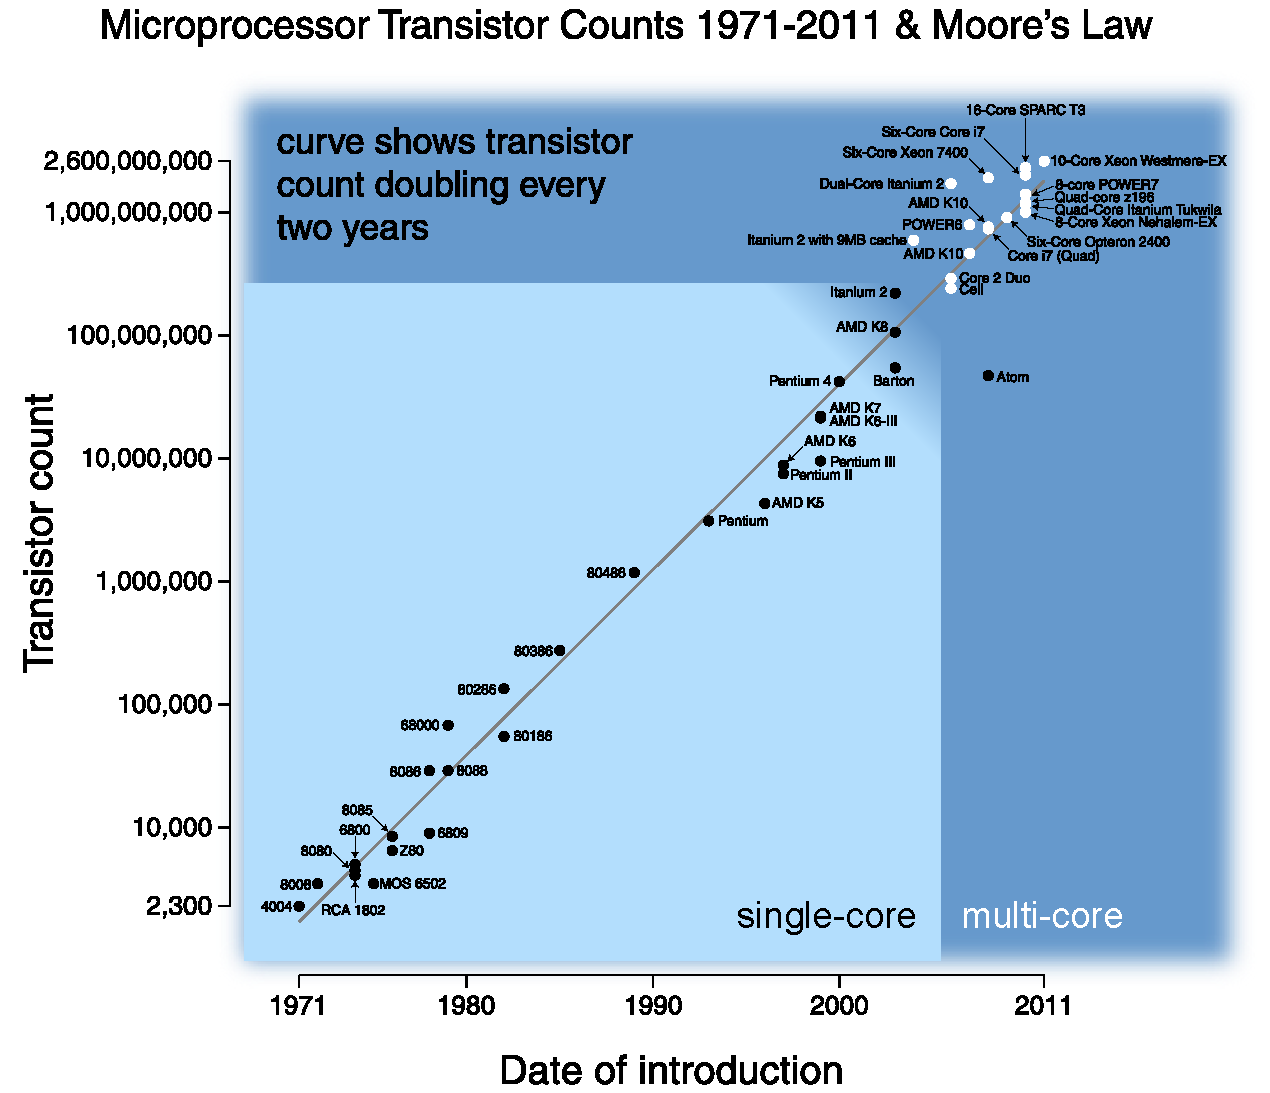
\includegraphics[width=\textwidth]{images/moore-law.pdf}
   \caption{Cantidad de transistores en procesadores emblematicos desde 1971}
   \label{moore-law}
\end{figure}

Sin embargo, a medida que los transistores disminuyen su tama\~no, aumentan su disipaci\'on t\'ermica por unidad de superficie.
Esto limita la cantidad que se pueden ubicar en un circuito sin producir que este se comporte de manera err\'atica. 
El mismo motivo impide el crecimiento de frecuencia de reloj, uno de los principales motores de avance en eficiencia. 
Los problemas t\'ermicos han implicado que desde el 2002, la tasa de crecimiento de la performance de los monoprocesadores haya disminuido a un 20\% anual.
Consecuentemente, los principales fabricantes de procesadores han modificado el enfoque de investigaci\'on y dise\~no, empezando a hacerse m\'as y m\'as com\'un el uso de m\'ultiples procesadores por chip.

La preocupaci\'on por la disipaci\'on y el consumo energ\'etico insustentables han sido motivadores de dise\~nos con menor frecuencia de clock, pero aprovechando las a\'un crecientes densidades de transistores para incrementar las unidades de soporte. 
Esta estrategia ha resultado en que, en un CPU moderno, menos del 20\% de todos los transistores disponibles se utilicen para realizar c\'alculos.

Adicionalmente, las mejoras de performance debidas al paralelismo a nivel de instrucci\'on (mediante t\'ecnicas como ejecuci\'on fuera de \'orden, ejecuci\'on especulativa, \textit{pipelining}, etc.) han sido progresivamente menores. 
Actualmente, los esfuerzos invertidos en ese \'area se han concentrado en el paralelismo a nivel de datos (vectorizaci\'on) y paralelismo a nivel de tareas (multiprocesadores)~\cite{HennessyPatterson}.

Este enfoque en dise\~no de arquitecturas hacia otros tipos de paralelismo puede verse tanto en nuevos productos en las l\'ineas establecidas (por ejemplo los procesadores Intel i3, i5 e i7) as\'i como tambi\'en en nuevos desarrollos que apunten a c\'omputo de alta performance.
La revalorizaci\'on de las placas gr\'aficas (GPUs) para problemas de c\'omputo intensivo, y los desarrollos nuevos como la arquitectura MIC (\textit{Many Integrated Core Architecture}) de Intel son claros ejemplos de esta tendencia.

El impacto de este enfoque hacia m\'ultiples hilos de ejecuci\'on en paralelo en el desarrollo de aplicaciones es significativo. 
En simulaciones para las \'areas de biolog\'ia, medicina, qu\'imica o meteorolog\'ia es de invaluable utilidad minimizar los tiempos de ejecuci\'on, para permitir mejores implementaciones de los modelos utilizados, permitiendo realizar predicciones de mayor calidad. 
Aprovechar las nuevas arquitecturas multiprocesador requiere modificaciones en el c\'odigo que resultan no triviales, a diferencia del crecimiento en velocidad de \textit{clock} que no requer\'ia modificaciones en el dise\~no del programa. 
Los intentos de escribir programas que conviertan programas seriales (dise\~nados para un solo procesador) a paralelos, en lenguajes de prop\'osito general como C, C++ o Fortran, han sido relativamente infructosos \todo{ACA DEBERIAN IR ALGUNOS EJEMPLOS Y CITAS}.

El resultado es que es necesario trabajo a nivel de escritura del \textit{software} para utilizar multiples procesadores. 
La aparici\'on de nuevas herramientas ayudan al programador en esta tarea. 
Un ejemplo de esto es Nvidia CUDA~(\textit{Compute Unified Device Architecture}), que provee un lenguaje de programaci\'on unificado para el desarrollo de aplicaciones que exploten la arquitectura de unidades GPGPU~(\textit{General Purpose Graphical Processing Units}). 
Otros ejemplos los podemos ver en APIs y librer\'ias unificadas de desarrollo como OpenMP o MPI~(\textit{Message Passing Interface}), trabajando conjuntamente con compiladores
optimizantes como Intel ICC y PGI Fortran.

Estas herramientas, si bien resultan en una asistencia muy importante para el programador, no son \textit{silver bullets}. 
Todav\'ia la divisi\'on del trabajo es inherente al problema a resolver, en base a las dependencias de las tareas a realizar para la soluci\'on del mismo. 
Realizar esta divisi\'on es una labor que, hasta el d\'ia de hoy, se relega en el programador especializado.

En este trabajo, buscaremos comparar distintas arquitecturas de hardware y c\'omo las caracter\'isticas espec\'ificas de la simulaci\'on qu\'imica a realizar permiten o impiden paralelizaci\'on de trabajo empleando los distintos recursos que cada arquitectura provee.
